\chapter{Data Representation}
\label{chap:Data_representation}
\begin{figure}[H]
    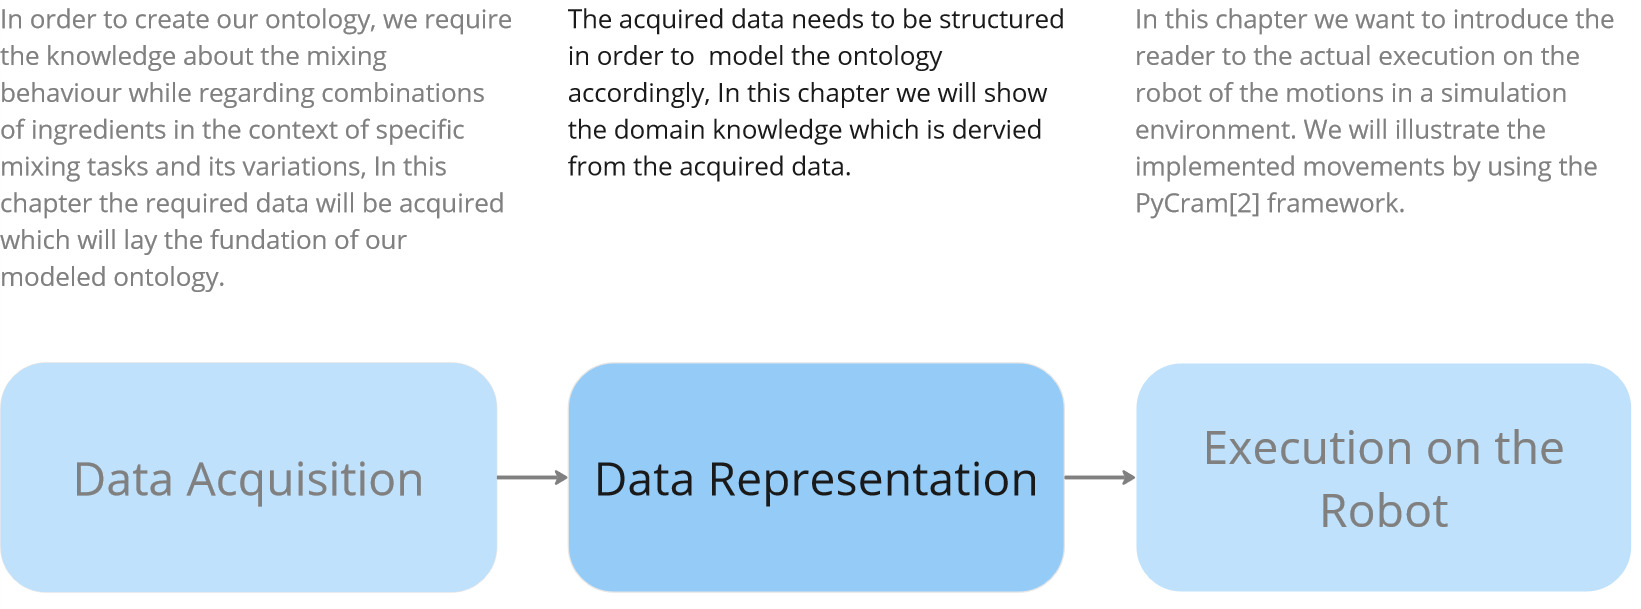
\includegraphics[scale=0.25]{Graphics/structure_overview2.jpg}
\end{figure} 
In this chapter we will present you the mixing knowledgegraph using \textit{OWL} as basis to formally define knowledge.
This knowledge base defines domain knowledge about mixing, which encompasses several aspects derived from the data acquisition.
Using assertional knowledge such as the task to execute, the set of ingredients as input for a mixing task, 
and additional knowledge like which container to use, the knowledge base can infer motions which should be executed via \textit{SWRL} rules.
Our goal is not to teach a robot how to execute a specific mixing motion, but rather infer a motion and relevant parameters for this motion. 
\newpage
\section{The Knowledgebase}
Our knowledgebase consists of the superclasses \textit{Ingrediet, DesginedTool, Task} and \textit{Motion}. These are the concepets which we dervied from the \nameref{chap:Data_acquisition}. The following image illustrates the \textit{Mixing} ontology hierarchy.
\begin{figure}[H]
    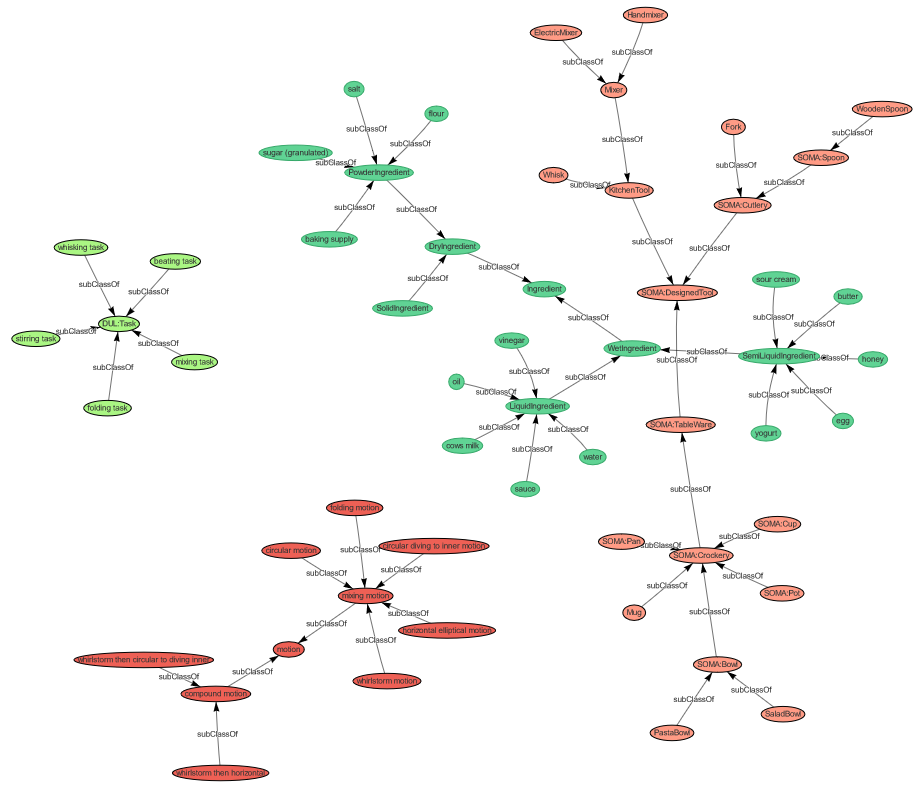
\includegraphics[scale=0.5]{Graphics/classHierarchy/taxonomy.png}
    \centering
    \caption{Mixing Ontology Taxonomy}
\end{figure}

\subsection{Ingredients}

\begin{figure}[H]
    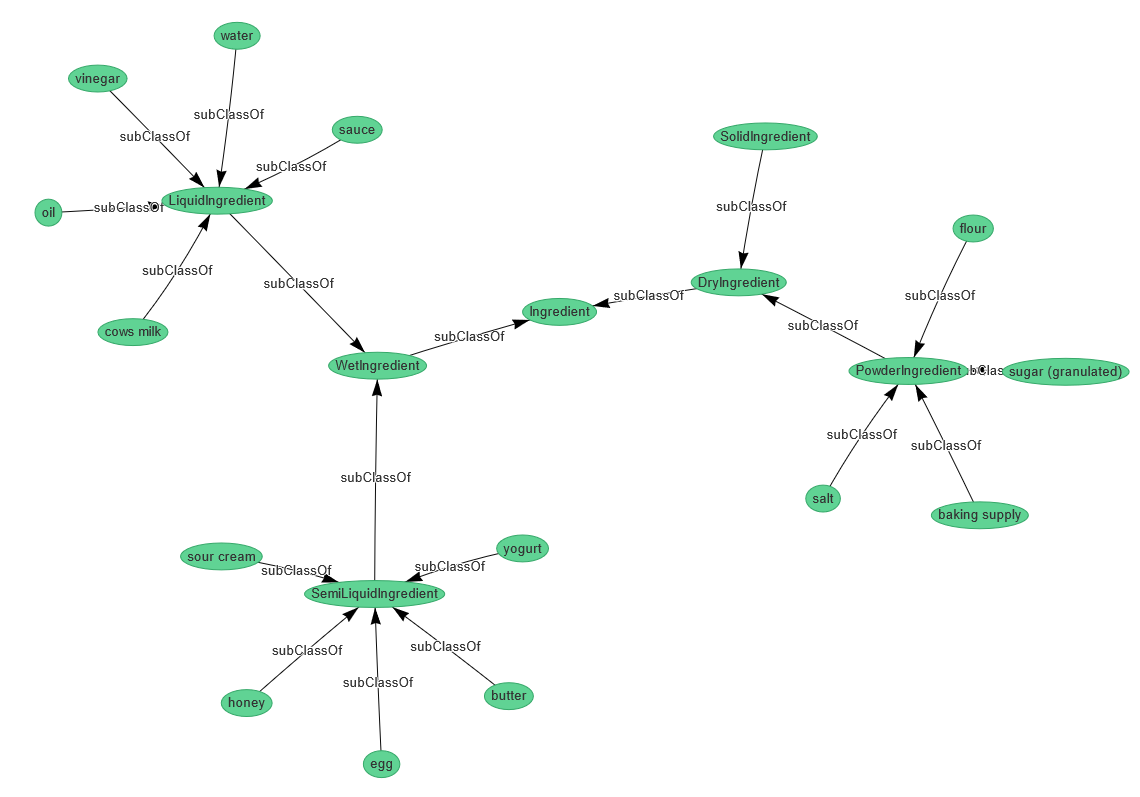
\includegraphics[scale=0.45]{Graphics/classHierarchy/ingredients_hierarchy.png}
    \centering
    \caption{Ingredients Hierarchy in Mixing Ontology}
\end{figure}

Ingredients are primarily divided into \textit{Dry} and \textit{Wet}, with a need for finer differentiation.
Wet ingredients can be further differentiated into \textit{Liquid} and \textit{Semi-Liquid}, where liquids include examples like water and semi-liquids include examples like egg whites or yolks. 
Dry ingredients, on the other hand, are divided into the subcategories \textit{Solid} and \textit{Powder}. 
Solid ingredients include whole vegetables and meat, while powder ingredients are not solid but rather granulated. 
This hierarchy of ingredients is modeled with a view towards the cooking domain and enables us to formulate rules to infer motions to perform. 
There does not exist a single hierarchy of ingredients, but rather many hierarchies modeling different aspects of ingredients.

\begin{itemize}
    \item \textit{Liquid: Milk, Oil, Water, Vinegar, Vanilla Extract, Sauces}.
    \item \textit{Semi-Liquid: Egg White, Egg yolk, Butter, Whipped Cream}.
    \item \textit{Powder: Flour, Salt, Sugar, Baking Soda, Cocoa Powder}.
    \item \textit{Solid: Onions, Pork, Chicken, Minced meat, Bacon}.
  \end{itemize}

For each specific ingredient, a respective \textit{FoodOn}\cite{dooley2018foodon} class is used. By using \textit{FoodOn}, we directly include all available subclasses of the 
\textit{FoodOn} class once the ontology is imported into the \textit{mixing} ontology.
Different variations of the same ingredient are then covered in case a finer differentiation is needed. 
Extending the hierarchy of ingredients can be done by for example integrating \textit{FoodOn} classes.  

\subsection{Tools and containers}
\label{sec:toolsandcontainers}

\begin{figure}[H]
    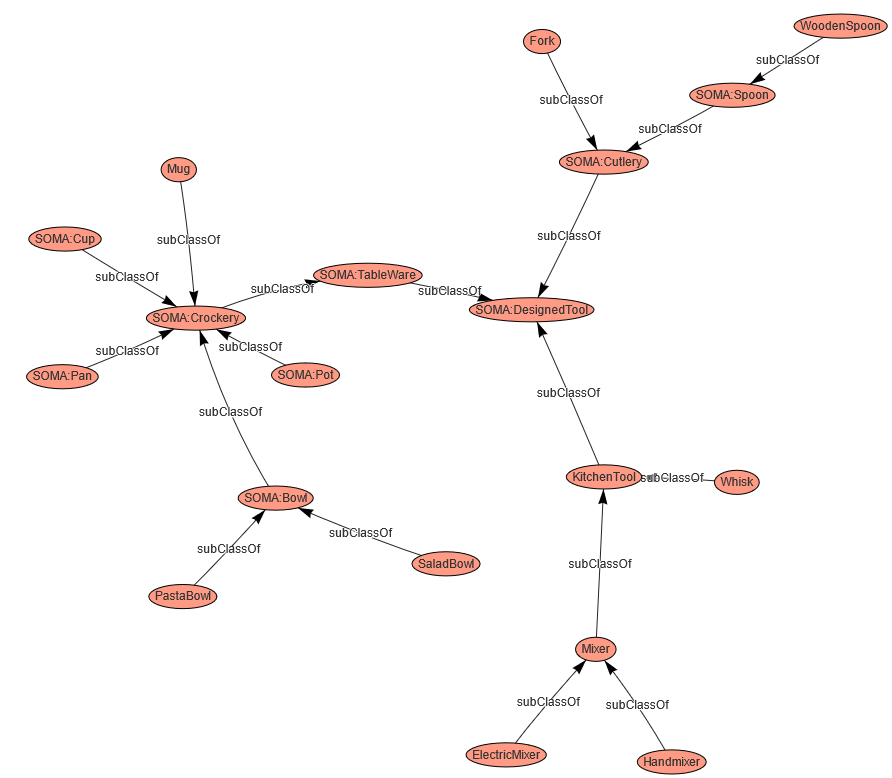
\includegraphics[scale=0.45]{Graphics/classHierarchy/tools_hierarchy.png}
    \centering
    \caption{Tools and Container Hierarchy in Mixing Ontology}
\end{figure}

Using the identified tools and containers from the data acquisition, we partially use \textit{SOMA} \cite{soma} to define parts of the containers and tools hierarchy.
We use the class \textit{DesignedTool} from \textit{SOMA-Home}, which consists of all kinds of container and tool classes. 
\textit{Crockery}, which is subsumed by \textit{DesignedTool}, is included with each container we identified. 
To include all kinds of cutlery, we use the class \textit{Cutlery}, which subsumes the classes \textit{Fork} and \textit{Spoon}. 
Mixers and whisks are not represented in \textit{SOMA-Home}, so we introduce a new class, \textit{KitchenTool}, which includes both of these tools.

Using \textit{SOMA-Home} has a few advantages:
\begin{enumerate}
    \item Using an existing hierarchy can be reused in other taxonomies.
    \item If \textit{SOMA-Home} is extended with new containers and tools, these concepts can be easily included.
    \item The \textit{mixing} ontology can be used by \textit{Soma-Home}, because both ontologies share classes.
\end{enumerate}

\subsection{Tasks}

\begin{figure}[H]
    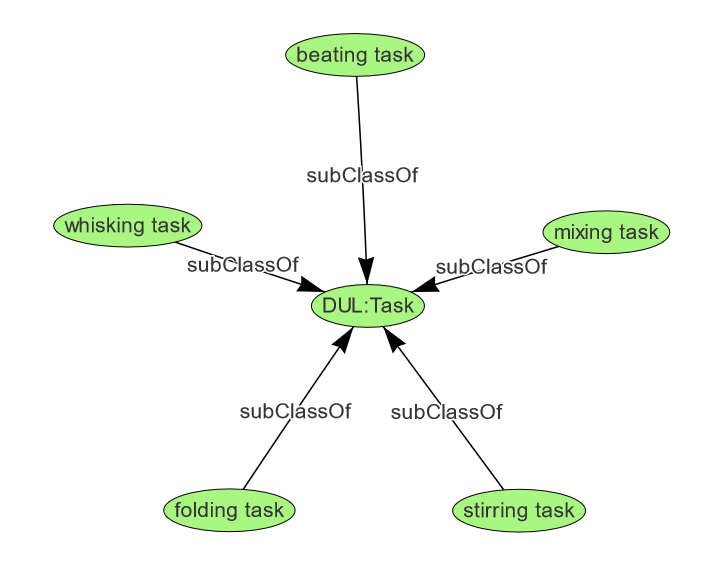
\includegraphics[scale=0.45]{Graphics/classHierarchy/task_hierarchy.png}
    \centering
    \caption{Task Hierarchy in Mixing Ontology}
\end{figure}

Mixing tasks are subclasses of the \textit{Task} superclass, where \textit{Task} is a \textit{DUL} concept. 
All variations of mixing tasks, which were acquired during our data acquisition, are included in the superclass \textit{Task}. 
These tasks include Stirring, which mostly involves a circular motion, Beating, which is mainly used in the context of eggs and other wet ingredients, 
Folding, which represents a gentle type of mixing, and Whisking, which is similar to beating. 
While some of these tasks have only one motion associated with them, like the Folding task, 
we discovered that the other tasks can have multiple motions associated with them. 
This decision is influenced by the set of ingredients on which the motion will be performed.

\subsection{Motions}
\begin{figure}[H]
    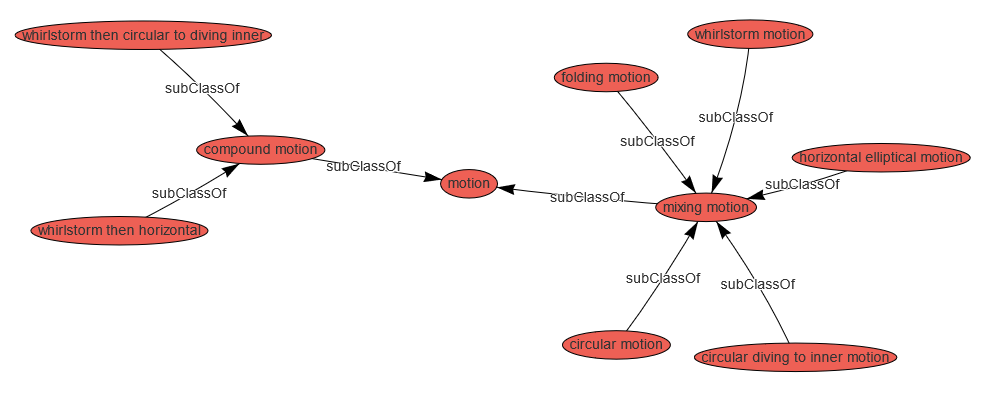
\includegraphics[scale=0.45]{Graphics/classHierarchy/motions_hierarchy.png}
    \centering
    \caption{Motion Hierarchy in Mixing Ontology}
\end{figure}

The top level class \textit{Motion} is the class of all possible motions which can be performed. MixingMotion a subclass of motion, are all mixing motions 
which were found during data acquisiton. To make a distinction between one singular mixing motion and motions consisting of at least two motions
we created the class \textit{CompoundMotions}, which defines a sequence of motions to be performed.
\textit{MixingMotion} is comprised of the following motions:

\begin{itemize}
    \item \textit{Circular Motion}: Simple Circular Motion
    \item \textit{Circular Diving To Inner}: Circular Motions including diving moving to the center of a container
    \item \textit{Folding Motion}: Motion executed as line with back and forth on multiple areas inside the container.
    \item \textit{Horizontal Elliptical Motion}: Multiple ellipse motions around the container, which resembles mixing `wildly`
    \item \textit{Whirlstorm Motion}: Whirlstorm or spiral like motion
\end{itemize}

Each motion has class restrictions with different kinds of motion parameters.

The following motion parameters are modelled in the \textit{mixing} ontology:

\begin{itemize}
    \item \textit{Radius lower Bound Relative}: The smallest possible radius relative to an object.
    \item \textit{Radius Upper Bound Relative}: The maximum possible radius relative to an object.
    \item \textit{Folding Rotation Shift}: An angle value of how much the folding line has to be rotated around .
    \item \textit{Repetetive Folding Rotation Shift}: After the folding motion has been executed this parameter rotates all folding lines.
     to cover similar areas of a container. 
    \item \textit{Ellipse Shift}: How much the ellipse has to be moved in meters. For example, if the ellipse shift is 0.04, then the ellipse
     is shifted 4 cm in the positive or negative direction along the x or y axes.
\end{itemize}

\textit{CompoundMotion} is comprised of the following classes:
\begin{itemize}
    \item \textit{WhirlstormThenCircularDivingToInner}: Execute whirlstorm motion followed by circular diving to inner motion.
    \item \textit{WhirlstormThenHorizontal}: Execute whirlstorm motion followed by horizontal elliptical motion.
\end{itemize}

Each of these compound motions have an OWL expression stating which motion is executed and which motions if following:

\[
	\begin{aligned}
	&\text{Motion}\\
    &\text{ and (hasMotion some}\\
    &\text{      (WhirlstormMotion}\\
    &\text{       and (followedBy some HorizontalEllipticalMotion)}\\
	&\text{     and (followedBy exactly 1 Motion)))}\\
	\end{aligned}
\]

This compound motion is equivalent to a \textit{Motion}, which has a motion \textit{WhirlstormMotion} followed by 
\textit{HorizontalEllipticalMotion}, where \textit{WhirlstormMotion} is exactly followed by one motion. 

How each of these motions is related to a task and the set of ingredients will be explained in the next section.

\section{Rules}
In order to infer the right motion based on the ingredients and task input, rules have to be defined. This rules are \nameref{sec:SWRL}-rules.
In this section we want to illustrate the inference on a high level.
The rules can be thoguht as if conditions, which will then result in a motion, 
for example, if we regard the combination of the task \textit{Mixing} and the ingredient type \textit{Liquid}, we infer the motion \textit{Whirlstorm Motion}. 
This can be done for every task and ingredient combination. 
The inference can be illustrated with decision trees which will be shown in the following section for every task and ingredient type combination available. 

\subsection{Mixing}
\begin{figure}[H]
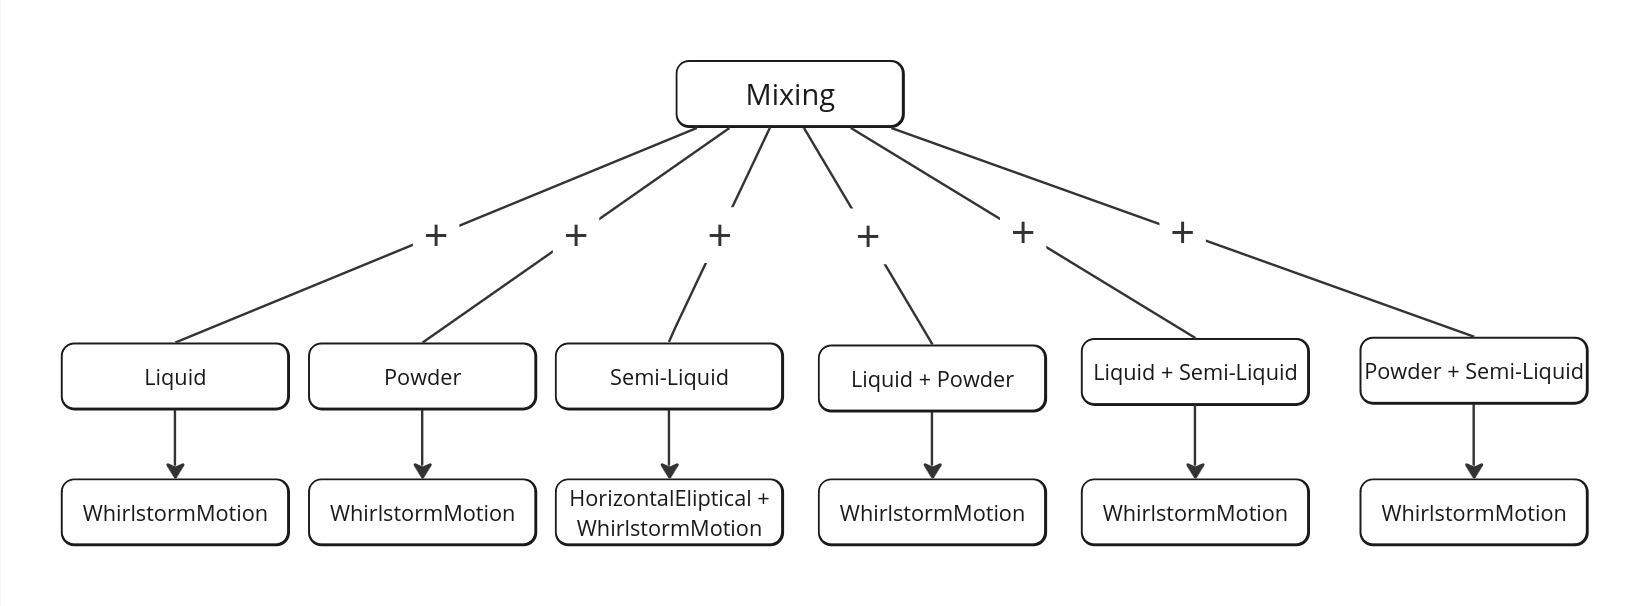
\includegraphics[scale=0.25]{Graphics/MixingDecisionTree.jpg}
\caption{Mixing decision tree}
\end{figure}
\textbf{Definition:} In the context of baking or cooking, a mixing task refers to the process of combining multiple ingredients thoroughly to create a homogeneous mixture. The goal is to distribute the ingredients evenly, ensuring that each component contributes to the overall texture, flavor, and consistency of the final dish or baked good. Mixing is a fundamental step in many recipes and is essential for achieving a balanced and cohesive result.


As can be seen from the illustration, the mixing task can primarily be mapped to the Whirlstorm motion. This is not surprising when considering the definition, as this motion results in the uniform distribution of all ingredients in the container.
\subsection{Stirring}
\begin{figure}[H]
    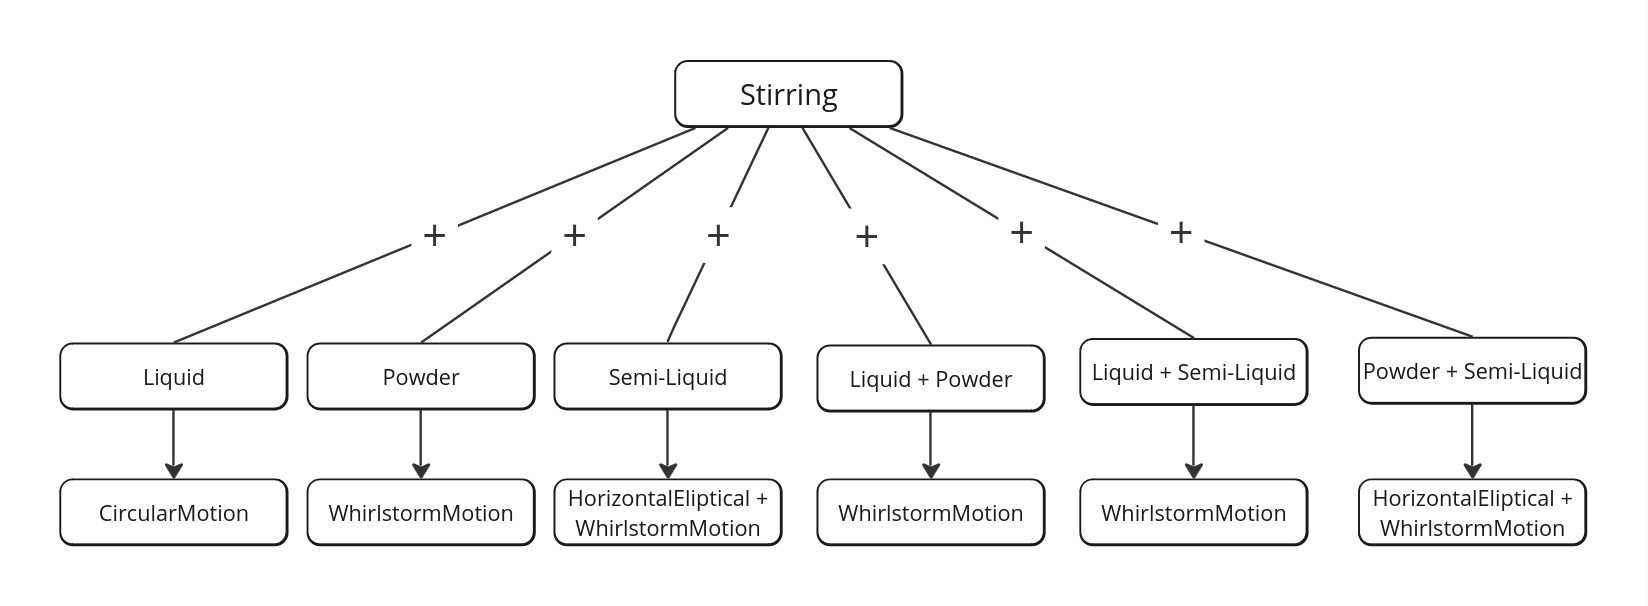
\includegraphics[scale=0.25]{Graphics/StirringDecisionTree.jpg}
    \end{figure}
\textbf{Definition:}
In the context of baking or cooking, a stirring task involves using a utensil, such as a spoon, spatula, or whisk, to agitate and circulate the ingredients within a mixture. The purpose of stirring is to achieve a uniform distribution of ingredients

In comparison to \textit{Mixing}, the \textit{Stirring} task, depending on the ingredients, maps to a broader range of motions. In addition to the \textit{Whirlstorm Motion}, the \textit{Circular Motion} is used here for the first time. This is particularly important when considering the \textit{Stirring} task with the ingredient type \textit{Liquid}, as one does not want the ingredients to be whirled, as would be the case with the \textit{Whirlstorm Motion}, but rather just stirred.
\subsection{Beating}
\begin{figure}[H]
    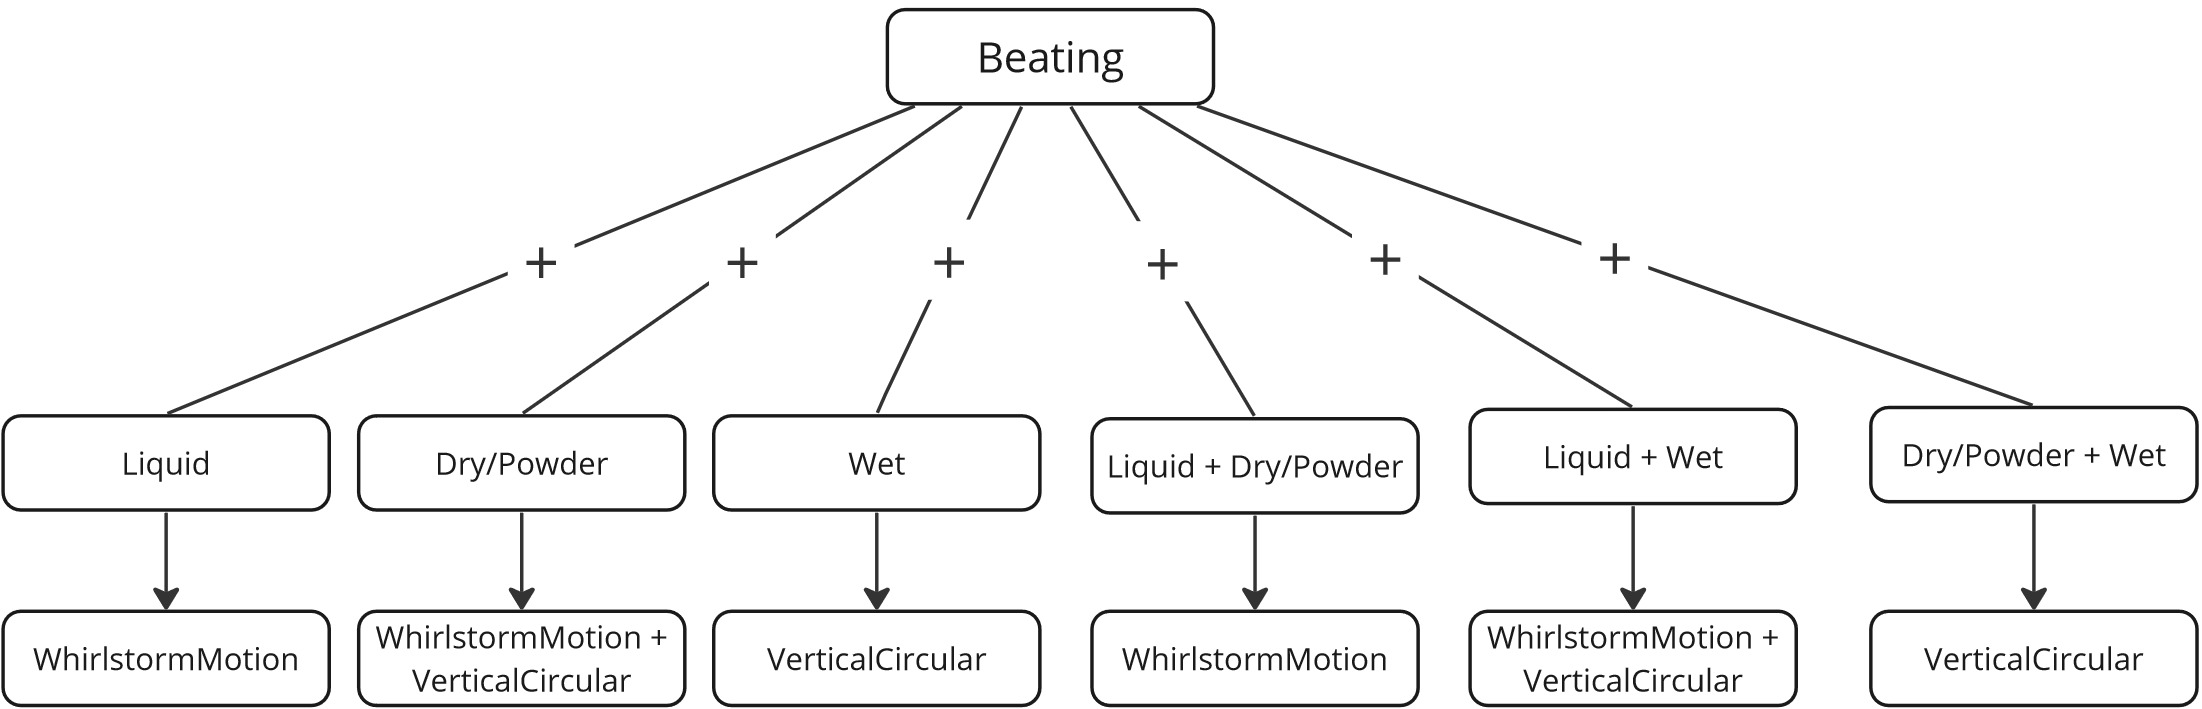
\includegraphics[scale=0.25]{Graphics/BeatingDecisionTree.jpg}
    \end{figure}
\textbf{Definition:}
In the context of baking and cooking, a \textit{Beating} task refers to the process of vigorously stirring or mixing ingredients to achieve a specific texture or consistency. \textit{Beating} is often done to incorporate air into the mixture, create smooth and uniform blends, or alter the physical properties of certain ingredients.

In addition to the \textit{Whirlstorm Motion}, the \textit{Horizontal Eliptic Motion} also predominates here. This can be derived from the definition as well, as this motion requires a wild mixing style, to which the \textit{Horizontal Eliptic Motion} aligns.
\subsection{Whisking}
\begin{figure}[H]
    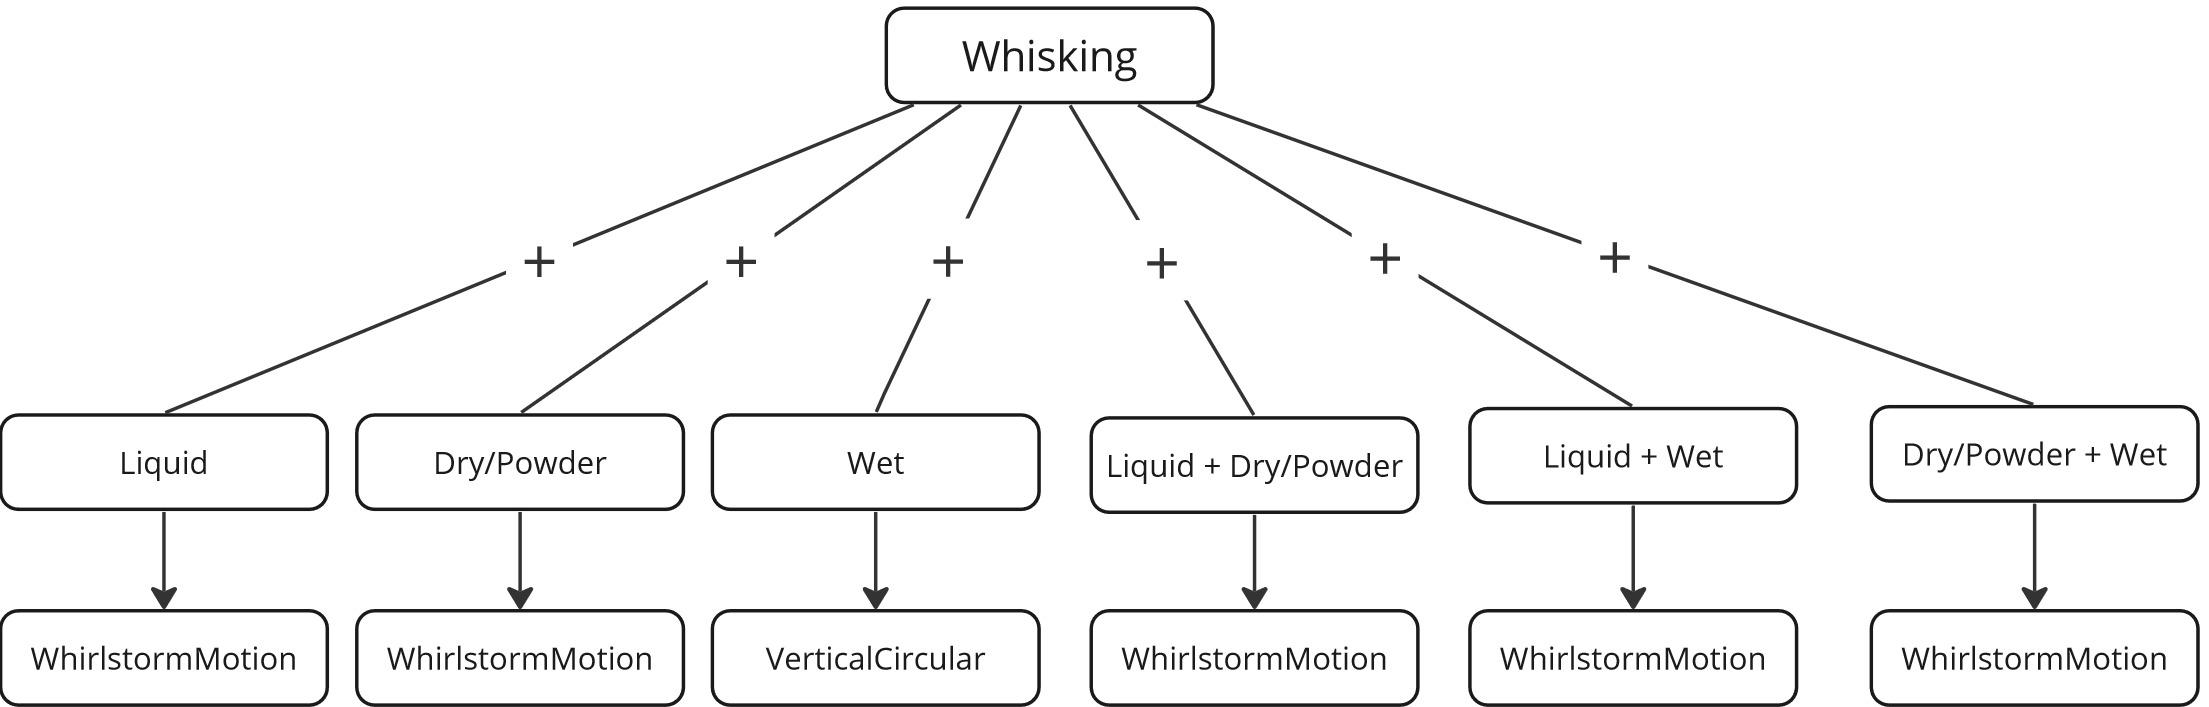
\includegraphics[scale=0.25]{Graphics/WhiskingDecisionTree.jpg}
    \end{figure}
\textbf{Definion:}In the context of baking and cooking, a \textit{Whisking} task involves using a kitchen utensil called a whisk to mix, blend, or beat ingredients. A whisk typically consists of wire loops or a coil attached to a handle, and it is designed to incorporate air into mixtures, break up clumps, and create a smooth and uniform texture.

\subsection{Folding}
\begin{figure}[H]
    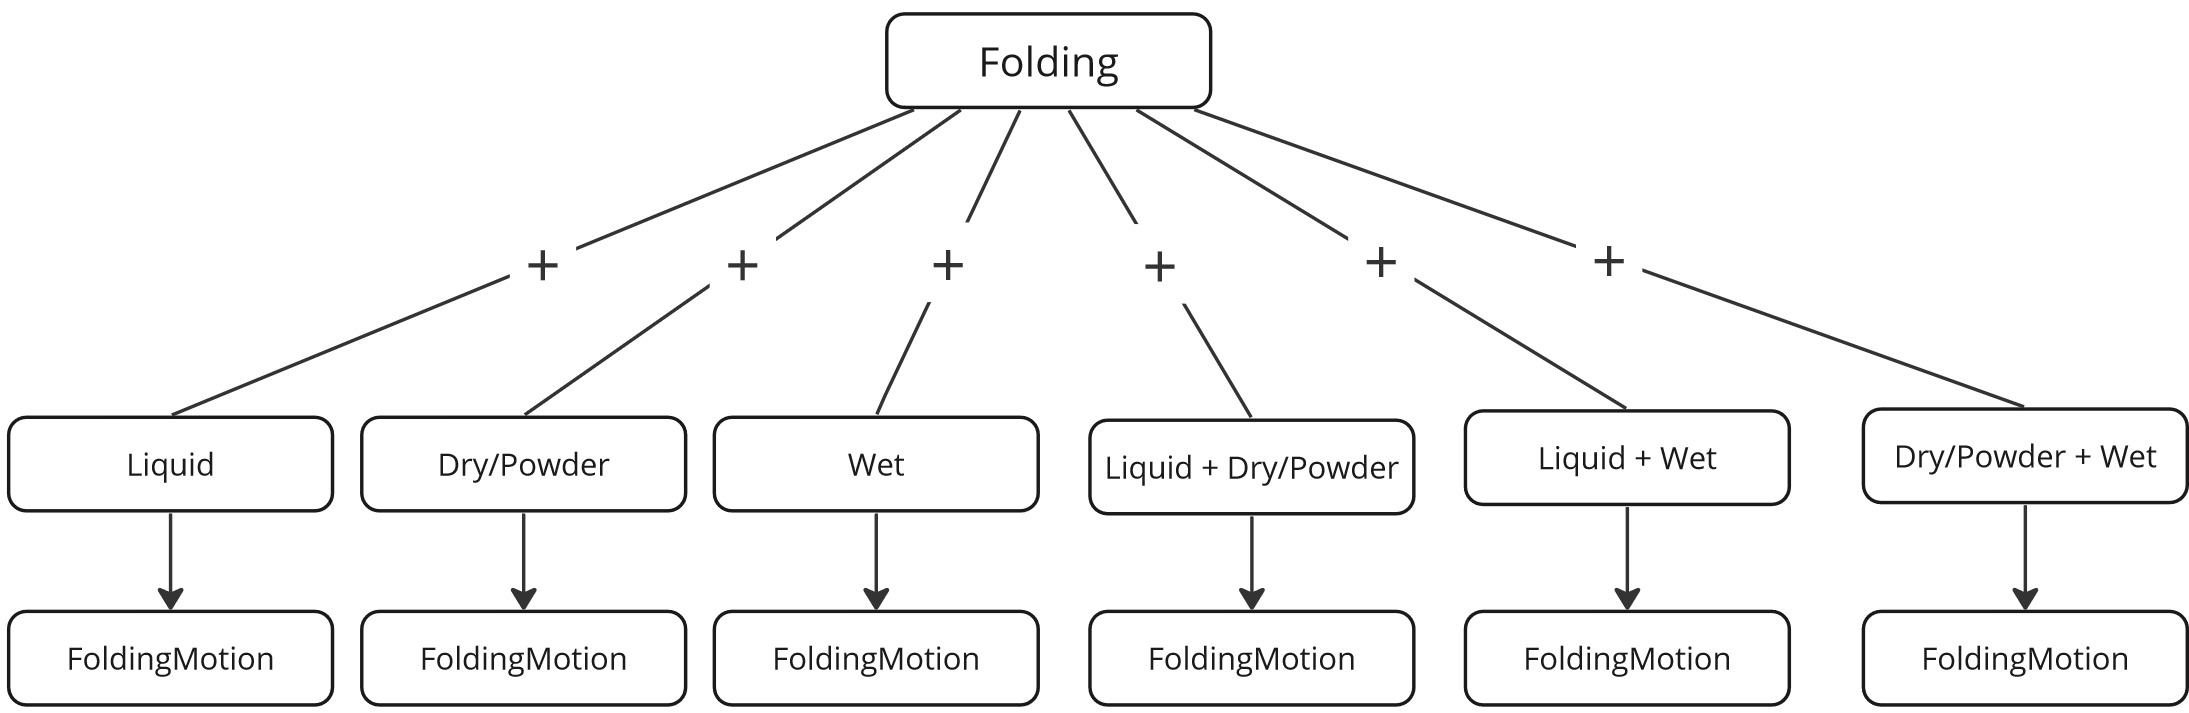
\includegraphics[scale=0.25]{Graphics/FoldingDecisionTree.jpg}
    \end{figure}
\textbf{Definition:}
In the context of baking and cooking, a \textit{Folding} task refers to a gentle mixing technique used to incorporate ingredients without deflating or destroying the air bubbles that have been created. \textit{Folding} is often employed when combining a lighter mixture (such as whipped cream or beaten egg whites) with a denser one (such as a batter or a heavier mixture). The goal is to maintain the desired texture, lightness, or fluffiness in the final dish.

Theoretically, we wouldn't need to graphically represent the \textit{Folding} Task since each task and ingredient combination maps to a single motion, the \textit{Folding} Motion. The graphic was nevertheless included for completeness. The \textit{Folding} Task requires a specific movement that does not remove the air in the mixture, and any other movement would fail.
